\iffalse
This file is protected by Copyright. Please refer to the COPYRIGHT file
distributed with this source distribution.

This file is part of OpenCPI <http://www.opencpi.org>

OpenCPI is free software: you can redistribute it and/or modify it under the
terms of the GNU Lesser General Public License as published by the Free Software
Foundation, either version 3 of the License, or (at your option) any later
version.

OpenCPI is distributed in the hope that it will be useful, but WITHOUT ANY
WARRANTY; without even the implied warranty of MERCHANTABILITY or FITNESS FOR A
PARTICULAR PURPOSE. See the GNU Lesser General Public License for more details.

You should have received a copy of the GNU Lesser General Public License along
with this program. If not, see <http://www.gnu.org/licenses/>.
\fi

%----------------------------------------------------------------------------------------
% Update the docTitle and docVersion per document
%----------------------------------------------------------------------------------------
\def\docTitle{OpenCPI\\ \bigskip ZedBoard Getting Started Guide}
\def\docVersion{1.4}
%----------------------------------------------------------------------------------------
\input{../../../../../../doc/av/tex/snippets/LaTeX_Header.tex}
\input{../../../../../../doc/av/tex/snippets/ocpidev_ide.tex}
\date{Version \docVersion} % Force date to be blank and override date with version
\title{\docTitle}
\lhead{Zedboard Getting Started Guide}
%----------------------------------------------------------------------------------------
\usepackage[T1]{fontenc} % http://tex.stackexchange.com/a/181119
\usepackage{graphicx}
\graphicspath{ {figures/} }
\lstset{ % https://tex.stackexchange.com/a/116572
  basicstyle=\ttfamily,
  columns=fullflexible,
  % frame=single,
  breaklines=true,
  showstringspaces=true,
  showspaces=true,
  postbreak=\mbox{\textcolor{red}{$\hookrightarrow$}\space},
}
\begin{document}
\maketitle
%\thispagestyle{fancy}

% AV-4173 blurb start
\begin{center}
\framebox{\parbox{0.8\linewidth}{\centering
\textcolor{red}{WARNING:}
Applications (including XML-only ones) fail if there is not an IP address assigned to the ZedBoard, even when in ``standalone mode.'' To set a temporary IP address, the command ``\code{ifconfig eth0 192.168.244.244}'' can be used. This problem was found late within the 1.4 release cycle and should be addressed with the next major release.
\PackageWarning{}{AV-4173} }}
\end{center}
% AV-4173 blurb end
\newpage

	\begin{center}
	\textit{\textbf{Revision History}}
		\begin{table}[H]
		\label{table:revisions} % Add "[H]" to force placement of table
			\begin{tabularx}{\textwidth}{|c|X|l|}
			\hline
			\rowcolor{blue}
			\textbf{Revision} & \textbf{Description of Change} & \textbf{Date} \\
		    \hline
		    v1.1 & Initial Release & 3/2017 \\
            \hline
            v1.2 & Updated for OpenCPI Release 1.2 & 8/2017 \\
            \hline
            v1.3 & Updated for OpenCPI Release 1.3 & 2/2018 \\
            \hline
            pre-v1.4 & Fixed inaccurate description for hardware jumper configuration, OpenCPI-SD-zed directory path, and MAC address modification instructions for multiple ZedBoards on the same network. & 4/2018 \\
            \hline
            v1.4 & Update descriptions and paths & 9/2018 \\
            \hline
			\end{tabularx}
		\end{table}
	\end{center}

\newpage

\tableofcontents

\newpage

\section{References}
	This document assumes a basic understanding of the Linux command line (or ``shell'') environment.  The reference(s) in Table 1 can be used as an overview of OpenCPI and may prove useful.
\def\refskipocpiov{}
\def\refcapbottom{}
\input{../../../../../../doc/av/tex/snippets/References_Table}

\newpage
\section{Overview}
This document provides steps for configuring a factory provided Digilent Zedboard with the OpenCPI run-time environment for executing applications, configuring a development system to build OpenCPI bitstreams targeting the \textit{zed} platform, and examples of executing applications on the OpenCPI configured Zedboard.

\section{Prerequisites}
\begin{flushleft}
This guide assumes that, at a minimum, the following RPMs are installed:  \\
\begin{table}[H]
	\label{table:rpms}
		\begin{tabularx}{\textwidth}{|c|X|}
		\hline
		\rowcolor{blue}
		\textbf{RPM Name} & \textbf{Description} \\
		\hline
		\hline
		All prerequisite RPMs & These packages have OpenCPI-specific patches and are provided as RPMs. This packaging ensures they will not conflict with other installed copies by using a nonstandard installation location of \path{/opt/opencpi/prerequisites}. \\
		\hline
		\small{\code{angryviper-ide-*.x86 64.rpm}} &
		The ANGRYVIPER IDE (Eclipse with plugins). See RPM Installation Guide.pdf, Appendix D for an alternative method to set up the IDE using an existing Eclipse installation. \\
		\hline
		\small{\code{opencpi-*.x86\_64.rpm}} &
		Base installation RPM includes the runtime portion of the Component
Development Kit (CDK) and the source for the ocpi.core and ocpi.assets Projects containing framework essential components, workers,
platforms, etc. \\
		\hline
		\small{\code{opencpi-devel-*.x86\_64.rpm}} &
		Additional header files and scripts for developing new assets as HDL
and/or RCC. \\
		\hline
		\small{\code{opencpi-sw-platform-xilinx13\_3-*.noarch.rpm}} &
		Additional files necessary to build the framework targeting specific
RCC/software platforms, independent of the final deployed hardware. \\
		\hline
		\small{\code{opencpi-hw-platform-zed-xilinx13\_3-*.noarch.rpm}} &
		Additional files necessary to build the framework targeting specific hardware platform ``X'' when running RCC platform ``Y'' (``Y'' can be ``no sw''). This RPM also includes hardware-specific SD Card images when applicable. \\
		\hline
	\end{tabularx}
\end{table}

\subsection{Installation of provided OpenCPI projects: \textit{core} and \textit{assets}}
This guide  assumes the user has executed \textit{ocpi-copy-projects}, accepting the default settings, to copy and register the \textit{core} and \textit{assets} projects from the /opt/opencpi/projects for building bitstreams for the Zedboard. Reference the Getting Started Guide for details on \textit{ocpi-copy-projects}.  While registering of the projects is performed during the execution of ocpi-copy-projects, changes to the registry can be made via \code{ocpidev un/register project} or the ANGRYVIPER GUI.\medskip

\begin{verbatim}
$ ocpi-copy-projects
...
$ ls ~/ocpi_projects
assets core
$ ocpidev show registry
Project registry is located at: /opt/opencpi/cdk/../project-registry
----------------------------------------------------------------------------------------
| Project Package-ID  | Path to Project                                 | Valid/Exists |
| ------------------  | ---------------                                 | ------------ |
| ocpi.core           | /home/user/ocpi_projects/core                   | True         |
| ocpi.assets         | /home/user/ocpi_projects/assets                 | True         |
----------------------------------------------------------------------------------------
\end{verbatim}

\subsection{Vendor Software Setup}
The platform that is expected to be used is the Digilent Zedboard (\textit{e.g.} zed). This OpenCPI-enabled platform provides the capability of deploying hardware and software workers while using Xilinx's 13.3 distribution of Linux.\\ \bigskip

The synthesizers and cross-compilers required to build HDL and RCC Workers for this platform are installed by following the instructions found in the \textit{OpenCPI FPGA Vendor Tools Installation Guide}. This document assumes that the user has installed the appropriate versions of Vivado and the Xilinx SDK.\\ \bigskip

\subsection{Building OpenCPI projects: \textit{core} and \textit{assets} }
\label{sec:Building OpenCPI projects}
The \textit{core} and \textit{assets} projects must be built \textit{in a specific order} for this platform. This section outlines how to build the relevant projects and provides the commands to do so.\medskip

For this document, the projects should be built as follows:\\

\begin{enumerate}
	\item Build \code{core} for the \code{xilinx13\_3} RCC Platform and the \code{zed} HDL Platform (approx 30 min)
	\item Build \code{assets} for the \code{xilinx13\_3} RCC Platform and the \code{zed} HDL Platform, but omit assemblies (approx 45 min)
	\item Build the \code{testbias} assembly from the \code{assets} project. This will be used later in this guide. (approx 10 min)
\end{enumerate}
\begin{lstlisting}[showspaces=false]
$ cd /home/<user>/ocpi_projects/
$ ocpidev build -d core     --rcc-platform xilinx13_3 --hdl-platform zed
$ ocpidev build -d assets   --rcc-platform xilinx13_3 --hdl-platform zed --no-assemblies
$ ocpidev build -d assets hdl assembly testbias       --hdl-platform zed
\end{lstlisting}
Note: replace ``\code{<user>}'' with your username in the commands above.\\\medskip

Each of these build commands can also be performed via the ANGRYVIPER IDE as follows:
\OcpidevBuild
See the ANGRYVIPER Team's Getting Started Guide for additional information concerning the use of \code{ocpidev} and the ANGRYVIPER IDE to build OpenCPI assets.

\subsection{Hardware Setup}
\begin{itemize}
\item \textbf{Digilent Zedboard}\\ \medskip
It is expected that this evaluation board includes a power supply, micro-USB to USB cable, micro-USB to female-USB adapter and standard SD card (4GB). \\ \medskip
OpenCPI has been tested on revisions C and D of the Zedboard. However, limitations have been observed for both revisions when used with the Zipper daughter card, details are provided in Myriad-RF\_1\_Zipper\_Limitations.pdf.\\ \medskip
The micro-USB serial port located on the top-side of the ZedBoard labeled UART, can be used to access the serial connection with the processor.\medskip

\begin{figure}[H]
	\centerline{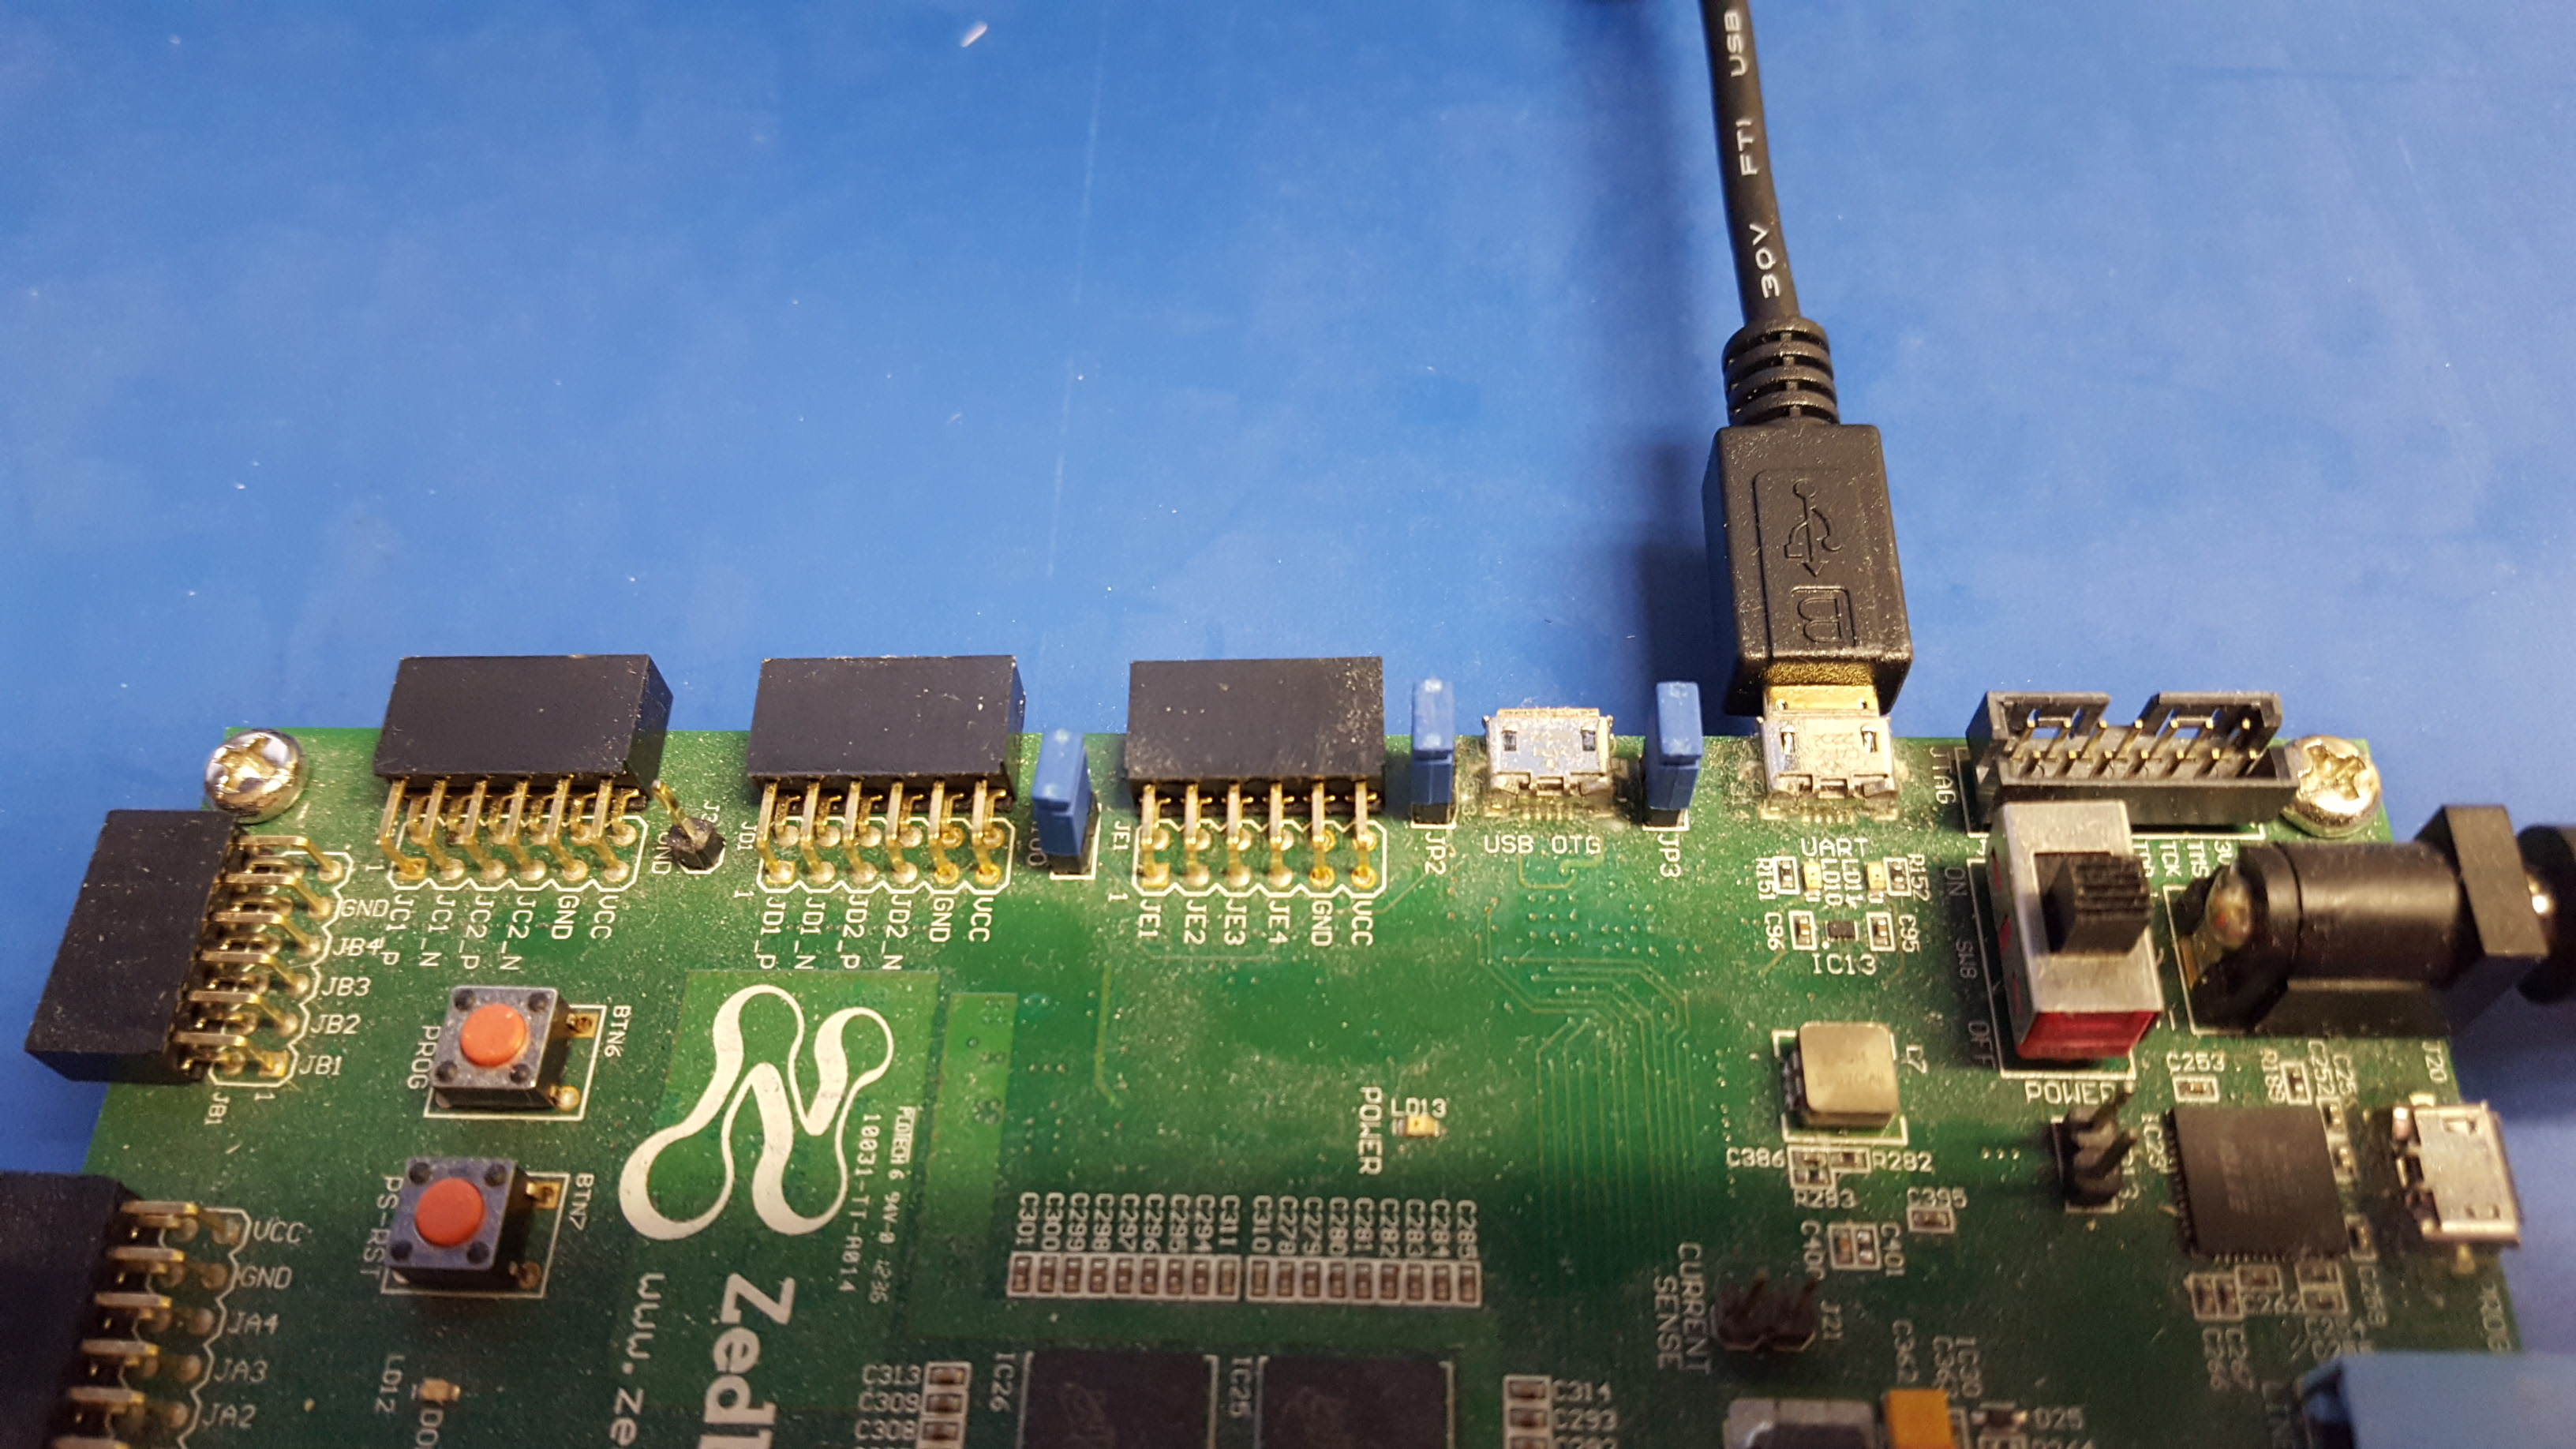
\includegraphics[scale=0.05]{zed_uart}}
	\caption{Connected Serial USB}
	\label{fig:zed_uart}
\end{figure}

Below the FMC LPC slot (bottom-side of the Zedboard), is the SD card slot which will be used throughout this guide.
\begin{figure}[H]
	\centerline{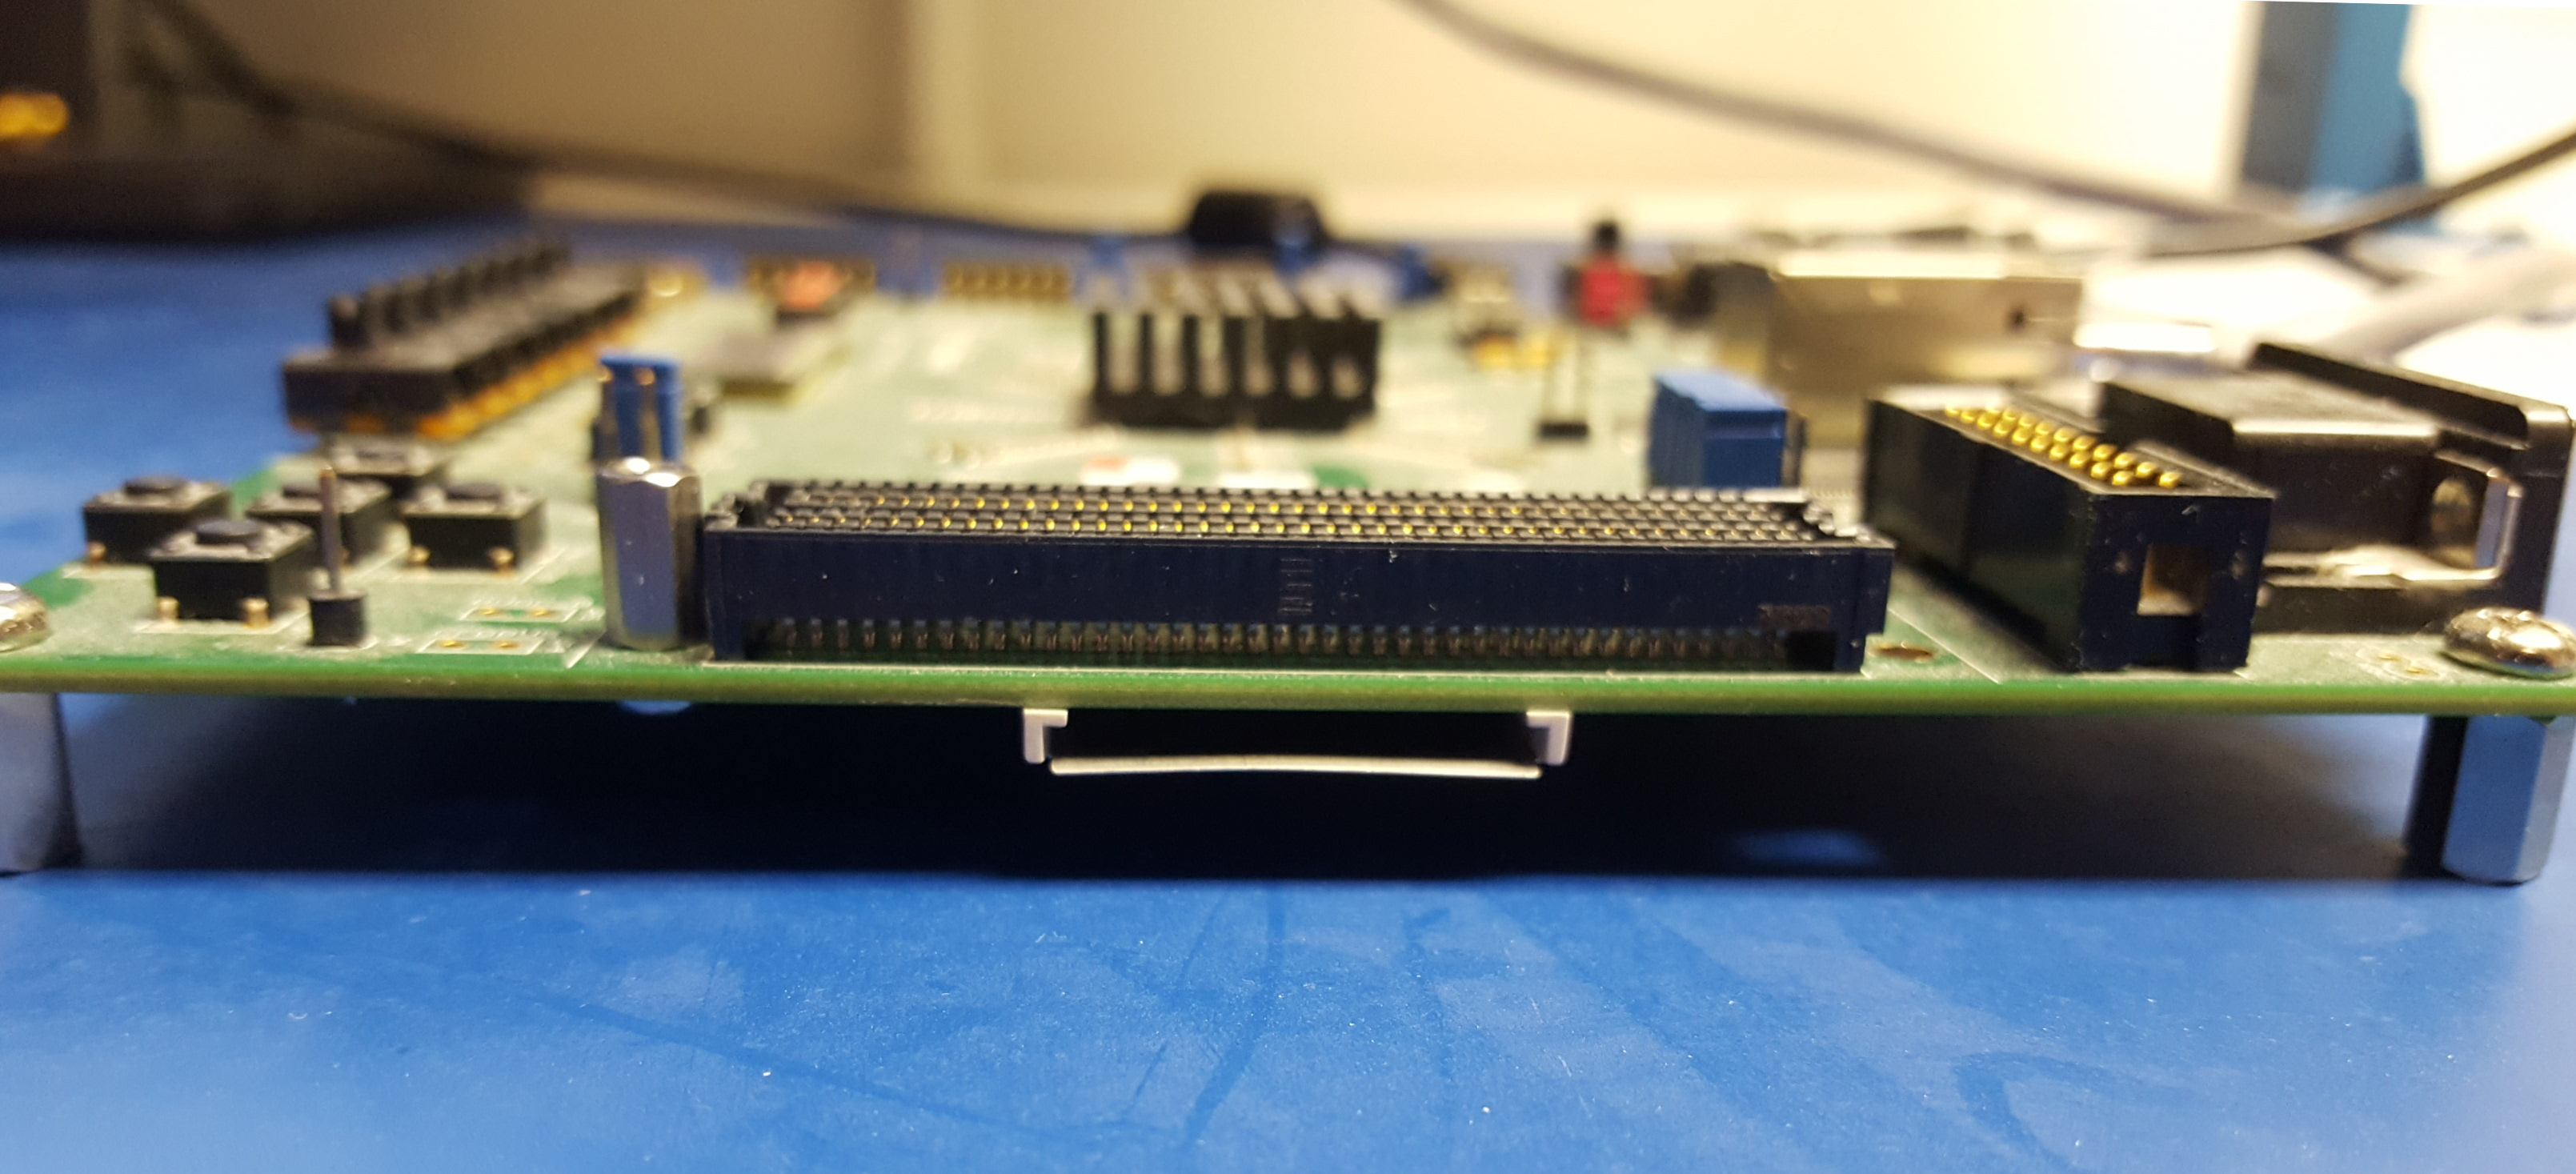
\includegraphics[scale=0.05]{zed_fmc_sd}}
	\caption{ZedBoard FMC Slot and SD card Slot}
	\label{fig:zed_fmc_sd}
\end{figure}

\item \textbf{Ethernet cable}:
An Ethernet port is available on the Zedboard and is required when the Network mode (discussed later) environment is used. The OpenCPI BSP for the ZedBoard is configured for DHCP.\medskip

\begin{figure}[H]
	\centerline{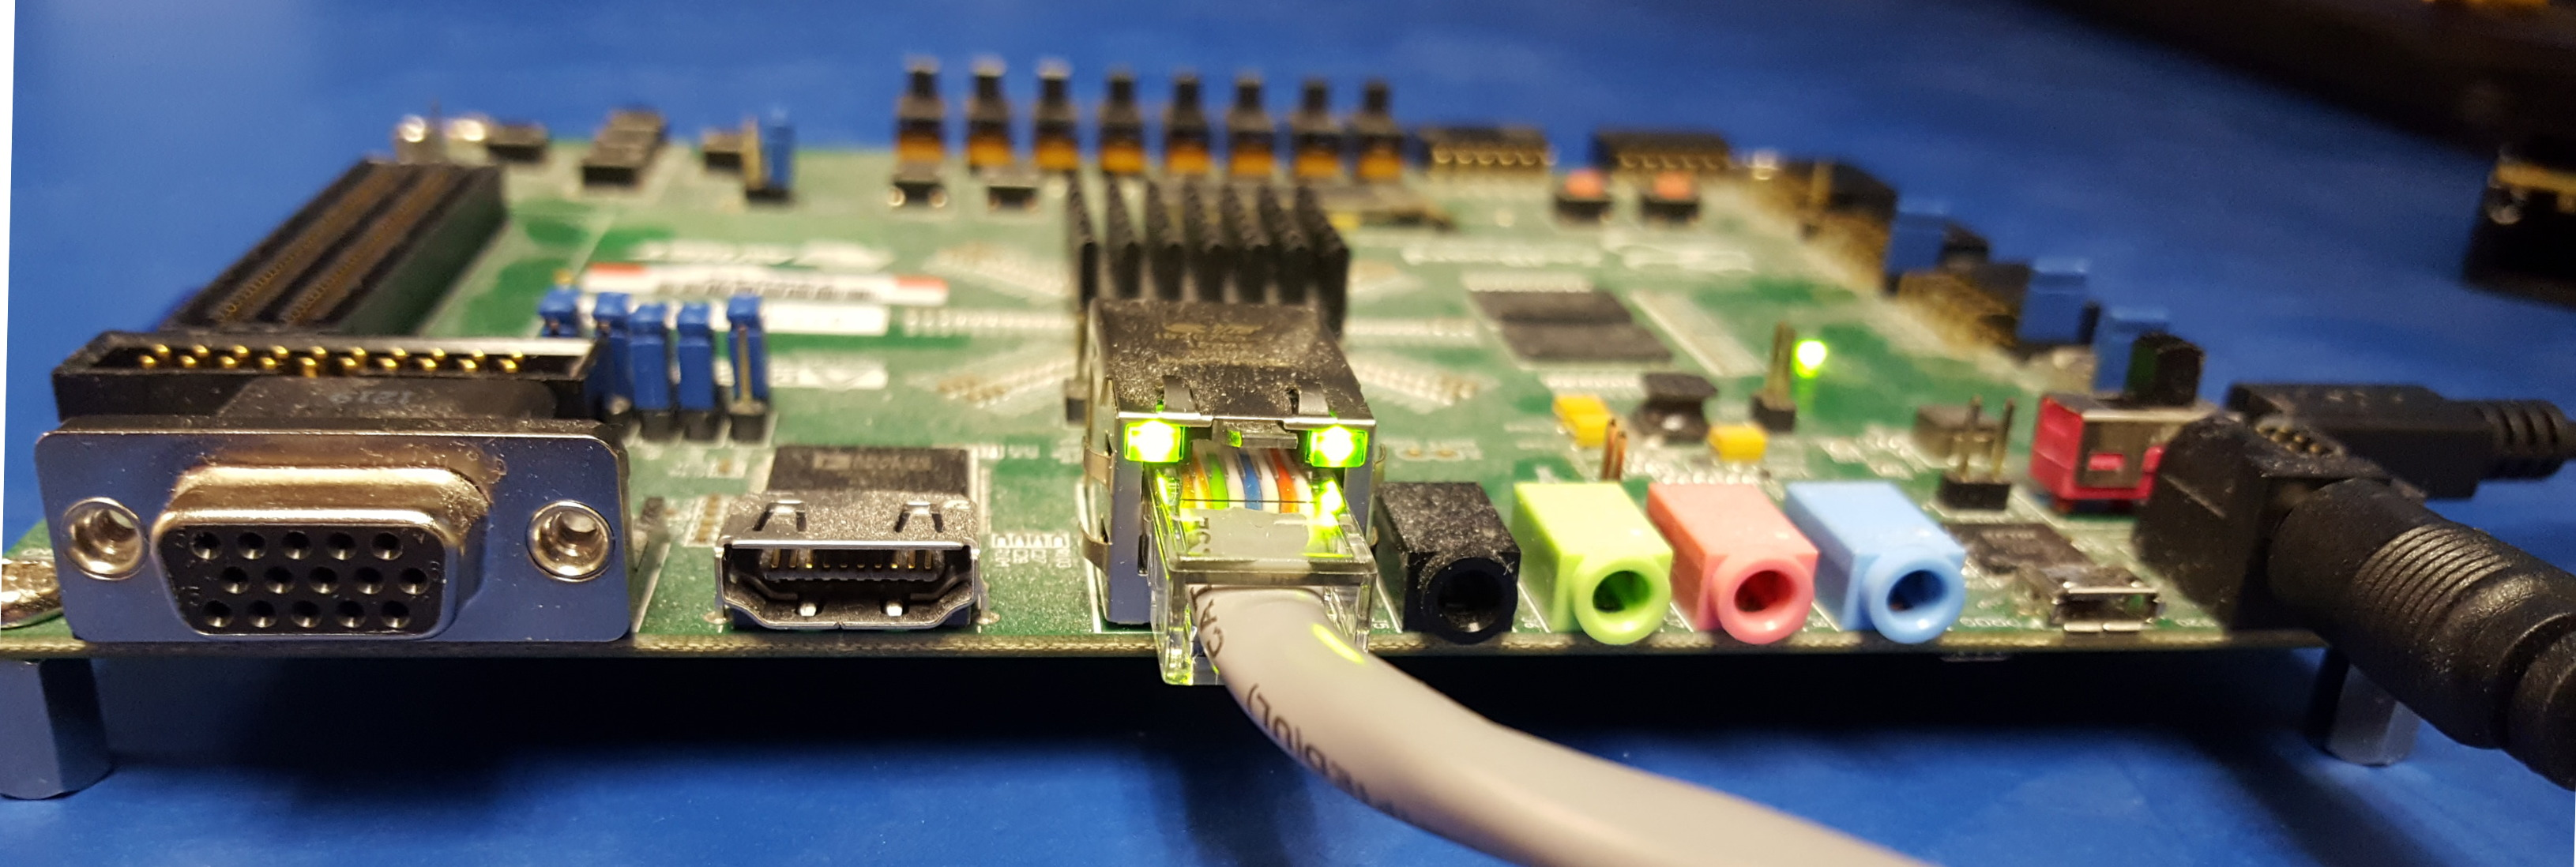
\includegraphics[scale=0.05]{zed_ether}}
	\caption{Connected Ethernet}
	\label{fig:zed_ether}
\end{figure}

\item \textbf{OpenCPI Zedboard BSP supported daughter cards (OPTIONAL)}\\
The ZedBoard has a FMC LPC slot that is used to connect plug-in modules or daughter cards. Currently, OpenCPI supports three FMC daughter cards, which may be installed on the Zedboard:
\begin{itemize}
	\item Analog Devices FMCOMMS2
	\item Analog Devices FMCOMMS3
	\item Lime Microsystems' Zipper card with the MyriadRF-1
\end{itemize} \medskip

\begin{figure}[ht]
	\centerline{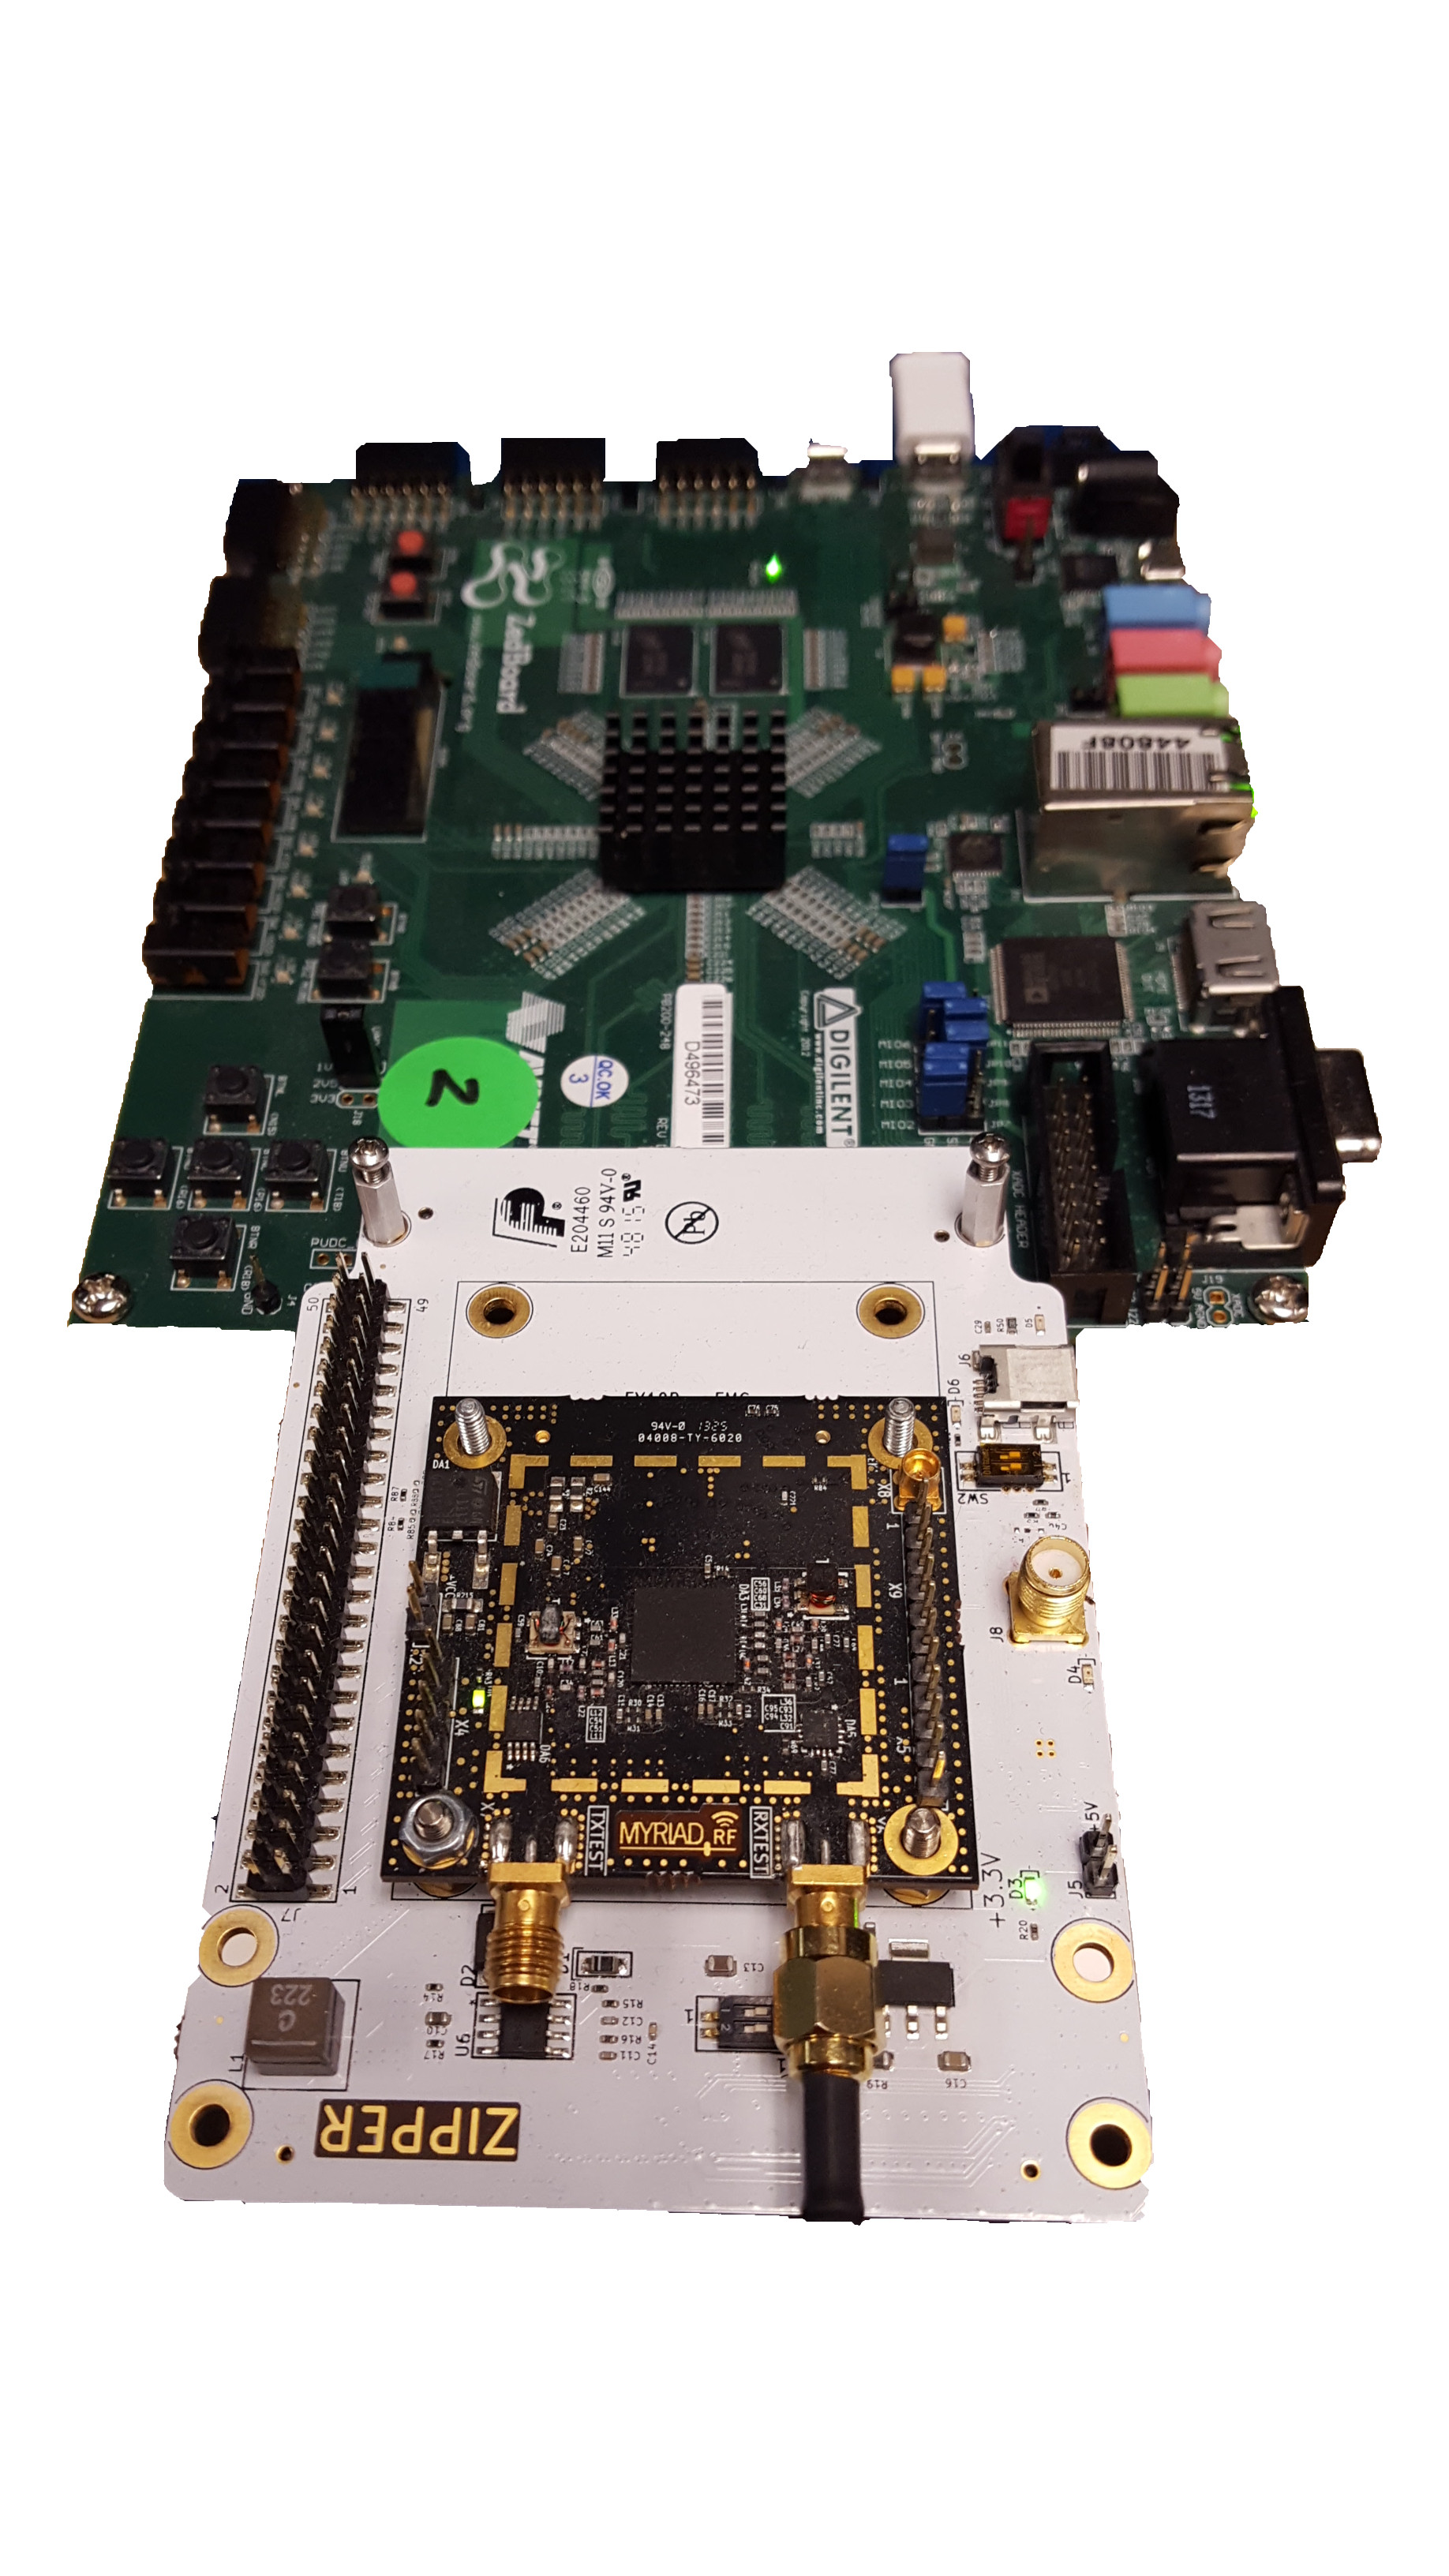
\includegraphics[scale=0.05]{zed_zipper}}
	\caption{ZedBoard With Zipper and MyriadRF-1 Connected to the FMC Slot}
	\label{fig:zed_zipper}
\end{figure}

\item \textbf{Access to a network which supports DHCP. (Network Mode)}

\item \textbf{SD card reader}
\end{itemize}
\end{flushleft}

\pagebreak
\section{SD Card Setup}
\label{sec:SD_Card_Setup}
\subsection{Make a backup image of factory SD card (assumes Linux host)}
This section provides the steps for creating an SD card backup image. It is optional, because the factory provided SD card does not have special formatting or content that must be preserved, unlike other systems (Epiq Solutions Matchstiq-Z1) that have been enabled for OpenCPI. The subsequent subsections assume the SD card is empty.

\begin{itemize}
\item Determine the device file name for the SD card by executing dmesg command below. It will likely be something like \texttt{/dev/sdb} or \texttt{/dev/mmcblk0}.\\
\texttt{\$ dmesg | tail -n 15} \\
\item Run the following dd command to make a backup image, where DEVICENAME was determined above. This step should take $\sim15$ minutes depending on the card size.\\ \medskip
\texttt{\$ dd if=DEVICENAME of=backup.image}
\end{itemize}
\noindent To restore the card back to the original contents, run the command ``\texttt{dd of=DEVICENAME if=backup.image}''

\subsection{Format the SD card}
\begin{itemize}
\item If the user requires the SD card to be formatted, use a single FAT32 partition.
\end{itemize}

\subsection{Copy embedded OS and boot files to SD card}
\label{sec:Copy embedded OS and boot files to SD card}
WARNING: The user must ensure that the contents of the SD, match the version of the OpenCPI release that the artifacts were built against.\\

\noindent When using the factory SD card (with the proper formatting), all files can be ignored or deleted. Any files/directories copied to the SD card will appear at \texttt{/mnt/card} on the Zed.\\

\noindent Copy the following files/directories onto the SD card:
\begin{verbatim}
$ cp /opt/opencpi/cdk/zed/sdcard-xilinx13_3/boot.bin /run/media/<user>/<partition>/

$ cp /opt/opencpi/cdk/zed/sdcard-xilinx13_3/devicetree.dtb /run/media/<user>/<partition>/

$ cp /opt/opencpi/cdk/zed/sdcard-xilinx13_3/uImage /run/media/<user>/<partition>/

$ cp /opt/opencpi/cdk/zed/sdcard-xilinx13_3/uramdisk.image.gz /run/media/<user>/<partition>/
\end{verbatim}\medskip

\subsection{Copy files to SD card for desired Mode(s)}
As previously discussed, Standalone and Network modes offer trade-offs for configuring the run-time environment of the platform. The following sections provide instructions for copying specific files/directories to the SD card in support of these modes. For maximum flexibility and completion of this getting started guide, it is recommended that the SD card be configured to support both modes, as covered in the next sub-section. However, instructions for configuring the SD card for each mode separately, have also been provided.

\subsubsection{Standalone and Network Modes}
The SD can be setup to support both modes, as there is no conflict between the files/directories for either mode. To setup the SD to support both modes:\\

\noindent After performing the steps from \ref{sec:Copy embedded OS and boot files to SD card}, copy the entire \textit{opencpi} directory to the SD card.

\begin{verbatim}
$ cp -rL /opt/opencpi/cdk/zed/sdcard-xilinx13_3/opencpi /run/media/<user>/<partition>/

$ cp /home/<user>/ocpi_projects/assets/hdl/assemblies/testbias/container-testbias_zed_base/\
target-zynq/testbias_zed_base.bit.gz /run/media/<user>/<partition>/opencpi/xilinx13_3/artifacts/
\end{verbatim}

\subsubsection{Standalone Mode}
After performing the steps from \ref{sec:Copy embedded OS and boot files to SD card}, copy the entire \textit{opencpi} directory to the SD card, then copy the relevant bitstreams, artifacts into the \textit{artifacts} directory and application XMLs into the \textit{applications} directory. For this getting started guide, only one bitstream is required to be copied onto the SD cards, where as the required artifacts and application XML where copied to the SD along with the entire \textit{opencpi} directory.

\begin{verbatim}
$ cp -rL /opt/opencpi/cdk/zed/sdcard-xilinx13_3/opencpi /run/media/<user>/<partition>/

$ cp /home/<user>/ocpi_projects/assets/hdl/assemblies/testbias/container-testbias_zed_base/\
target-zynq/testbias_zed_base.bit.gz /run/media/<user>/<partition>/opencpi/xilinx13_3/artifacts/
\end{verbatim}

\subsubsection{Network Mode}
After performing the steps from \ref{sec:Copy embedded OS and boot files to SD card}, create a directory on the partition named \code{opencpi} and copy the following files into the this directory:

\begin{verbatim}
$ mkdir /run/media/<user>/<partition>/opencpi

$ cp /opt/opencpi/cdk/zed/sdcard-xilinx13_3/opencpi/default_mynetsetup.sh \
/run/media/<user>/<partition>/opencpi/

$ cp /opt/opencpi/cdk/zed/sdcard-xilinx13_3/opencpi/zynq_net_setup.sh \
/run/media/<user>/<partition>/opencpi/
\end{verbatim}

\subsection{SD Card Source}
The final SD Card artifacts are distributed in \path{/opt/opencpi/cdk/zed/} via RPM as noted previously. The end user is not required nor expected to generate the files.

\pagebreak
\section{Script Setup}
There are two type of setups or modes for running applications on any embedded radio: Network and Standalone. In Network mode, a development system hosts the OpenCPI tree as an NFS server to the ZedBoard which is an NFS client. This configuration provides quick and dynamic access to all of OpenCPI, and presumably any applications, components and bitstreams. In Standalone mode, all the artifacts are located on the SDR's local storage (\textit{e.g.} SD card) and no network connection is required. This may be more suited for \textit{deployment} scenarios in which network connection is not possible or practical. Network mode is generally preferred during the development process.

\begin{flushleft}

\subsection{Setting up the Network and Standalone Mode scripts}

For each mode, a startup script is used to configure the environment of the embedded system. The OpenCPI framework provides a default script for each mode. The default scripts are to be copied and modified per the user's requirements.\par\medskip

\subsubsection{Network Mode}
1) Make a copy of the default script for editing.
\begin{verbatim}
$ cp /run/media/<user>/<partition>/opencpi/default_mynetsetup.sh \
/run/media/<user>/<partition>/opencpi/mynetsetup.sh
\end{verbatim}\medskip

2) Edit the copy
\begin{enumerate}
\item In \texttt{mynetsetup.sh}, uncomment the following lines which are necessary for mounting \textit{core} and \textit{assets} project:

\begin{verbatim}
mkdir -p /mnt/ocpi_core
mount -t nfs -o udp,nolock,soft,intr $1:/home/user/ocpi_projects/core /mnt/ocpi_core
mkdir -p /mnt/ocpi_assets
mount -t nfs -o udp,nolock,soft,intr $1:/home/user/ocpi_projects/assets /mnt/ocpi_assets
\end{verbatim}
 \item Edit \texttt{/home/user/ocpi\_projects/core} and \texttt{/home/user/ocpi\_projects/assets} to reflect the paths to the \textit{core} and \textit{assets} project on the host, e.g.:
\begin{verbatim}
mkdir -p /mnt/ocpi_core
mount -t nfs -o udp,nolock,soft,intr $1:/home/johndoe/ocpi_projects/core /mnt/ocpi_core
mkdir -p /mnt/ocpi_assets
mount -t nfs -o udp,nolock,soft,intr $1:/home/johndoe/ocpi_projects/assets /mnt/ocpi_assets
\end{verbatim}
\end{enumerate}

\subsubsection{Standalone Mode}
In this mode, all OpenCPI artifacts that are required to run any application on the ZedBoard must be copied onto the SD card.  Building the provided projects to obtain such artifacts is discussed in Section \ref{sec:Building OpenCPI projects}. Once the artifacts have been created, they must be copied to the SD card in Section \ref{sec:SD_Card_Setup}. In general, any required \texttt{.so} (RCC workers), \texttt{.bit.gz} (hdl assemblies), and application XMLs or executables must be copied to the SD card.\medskip

1) Make a copy of the default script for editing\medskip
\begin{verbatim}
$ cp /run/media/<user>/<partition>/opencpi/default_mysetup.sh \
/run/media/<user>/<partition>/opencpi/mysetup.sh
\end{verbatim}\medskip

2) Edit the copy\\ \medskip
Unlike Network mode, there is no required modifications to this script. \medskip

3) Copy any additional artifacts to SD card's \path{opencpi/xilinx13_3/artifacts/} directory \medskip

\input{../../../../../../doc/av/tex/snippets/Setup_System_Time.tex}
\end{flushleft}

\subsection{Multiple ZedBoards on the same network}
\label{sec:Multiple ZedBoards on the same network}
If it is required that multiple ZedBoards are to be on the same network, the following change to the zynq startup scripts is required. This is necessary because by default the ZedBoards have the same MAC address from the factory. To resolve this, uncomment the following lines in the mynetsetup.sh and/or mysetup.sh scripts and modify the Ethernet address to be unique:
\begin{verbatim}
  # ifconfig eth0 down
  # ifconfig eth0 hw ether <unique MAC address> # e.g. ifconfig eth0 hw ether 00:0a:35:00:01:24
  # ifconfig eth0 up
  # udhcpc
\end{verbatim}

\pagebreak
\section{Hardware Setup}

\subsection{Establish a Serial Connection}
By default, the USB to Serial adapter connects as read-only, which requires sudo privileges for establishing a serial connection. OpenCPI recognizes that sudo may not be available and has provided an alternative for configuring the device thereby allowing all users access to the device. Specifically, this is accomplished by adding \texttt{udev} rules to instruct the device connection to have read and write permissions for all users.
\begin{itemize}
\item If OpenCPI was installed via RPMs, the \texttt{udev} rules are automatically setup for the user.
\item If OpenCPI was installed from source, then the user must manually add the \texttt{udev} rules by copying the file from the host machine's installation directory to the host machine's \path{/etc/udev/rules.d/}. The following command can be used as a guide:
\begin{verbatim}
$ cd /etc/udev/rules.d/
$ sudo ln -s /<install-path>/opencpi/cdk/zed/host-udev-rules/98-zedboard.rules 98-zedboard.rules
\end{verbatim}
\item Whether installed via RPMs or source (and manually creating the symbolic link), the USB to Serial adapter will be connected as \texttt{/dev/zed0} with read and write permissions for all users.
\end{itemize}

\noindent Once the Zedboard is powered on and micro-USB cable is connected UART to the development host, use the following command to connect to the serial port:
\begin{verbatim}
$ screen /dev/zed0 115200
\end{verbatim}
\medskip

\subsection{Booting the ZedBoard from the SD card}
\begin{enumerate}
\item Remove power from the ZedBoard unit.
\item Ensure jumpers are configured correctly
\begin{enumerate}
\item To boot from the SD card, jumpers JP10, JP9, and JP8 need to be set to 3.3V, 3.3V, and GND respectively as shown below.
\begin{figure}[ht]
	\centerline{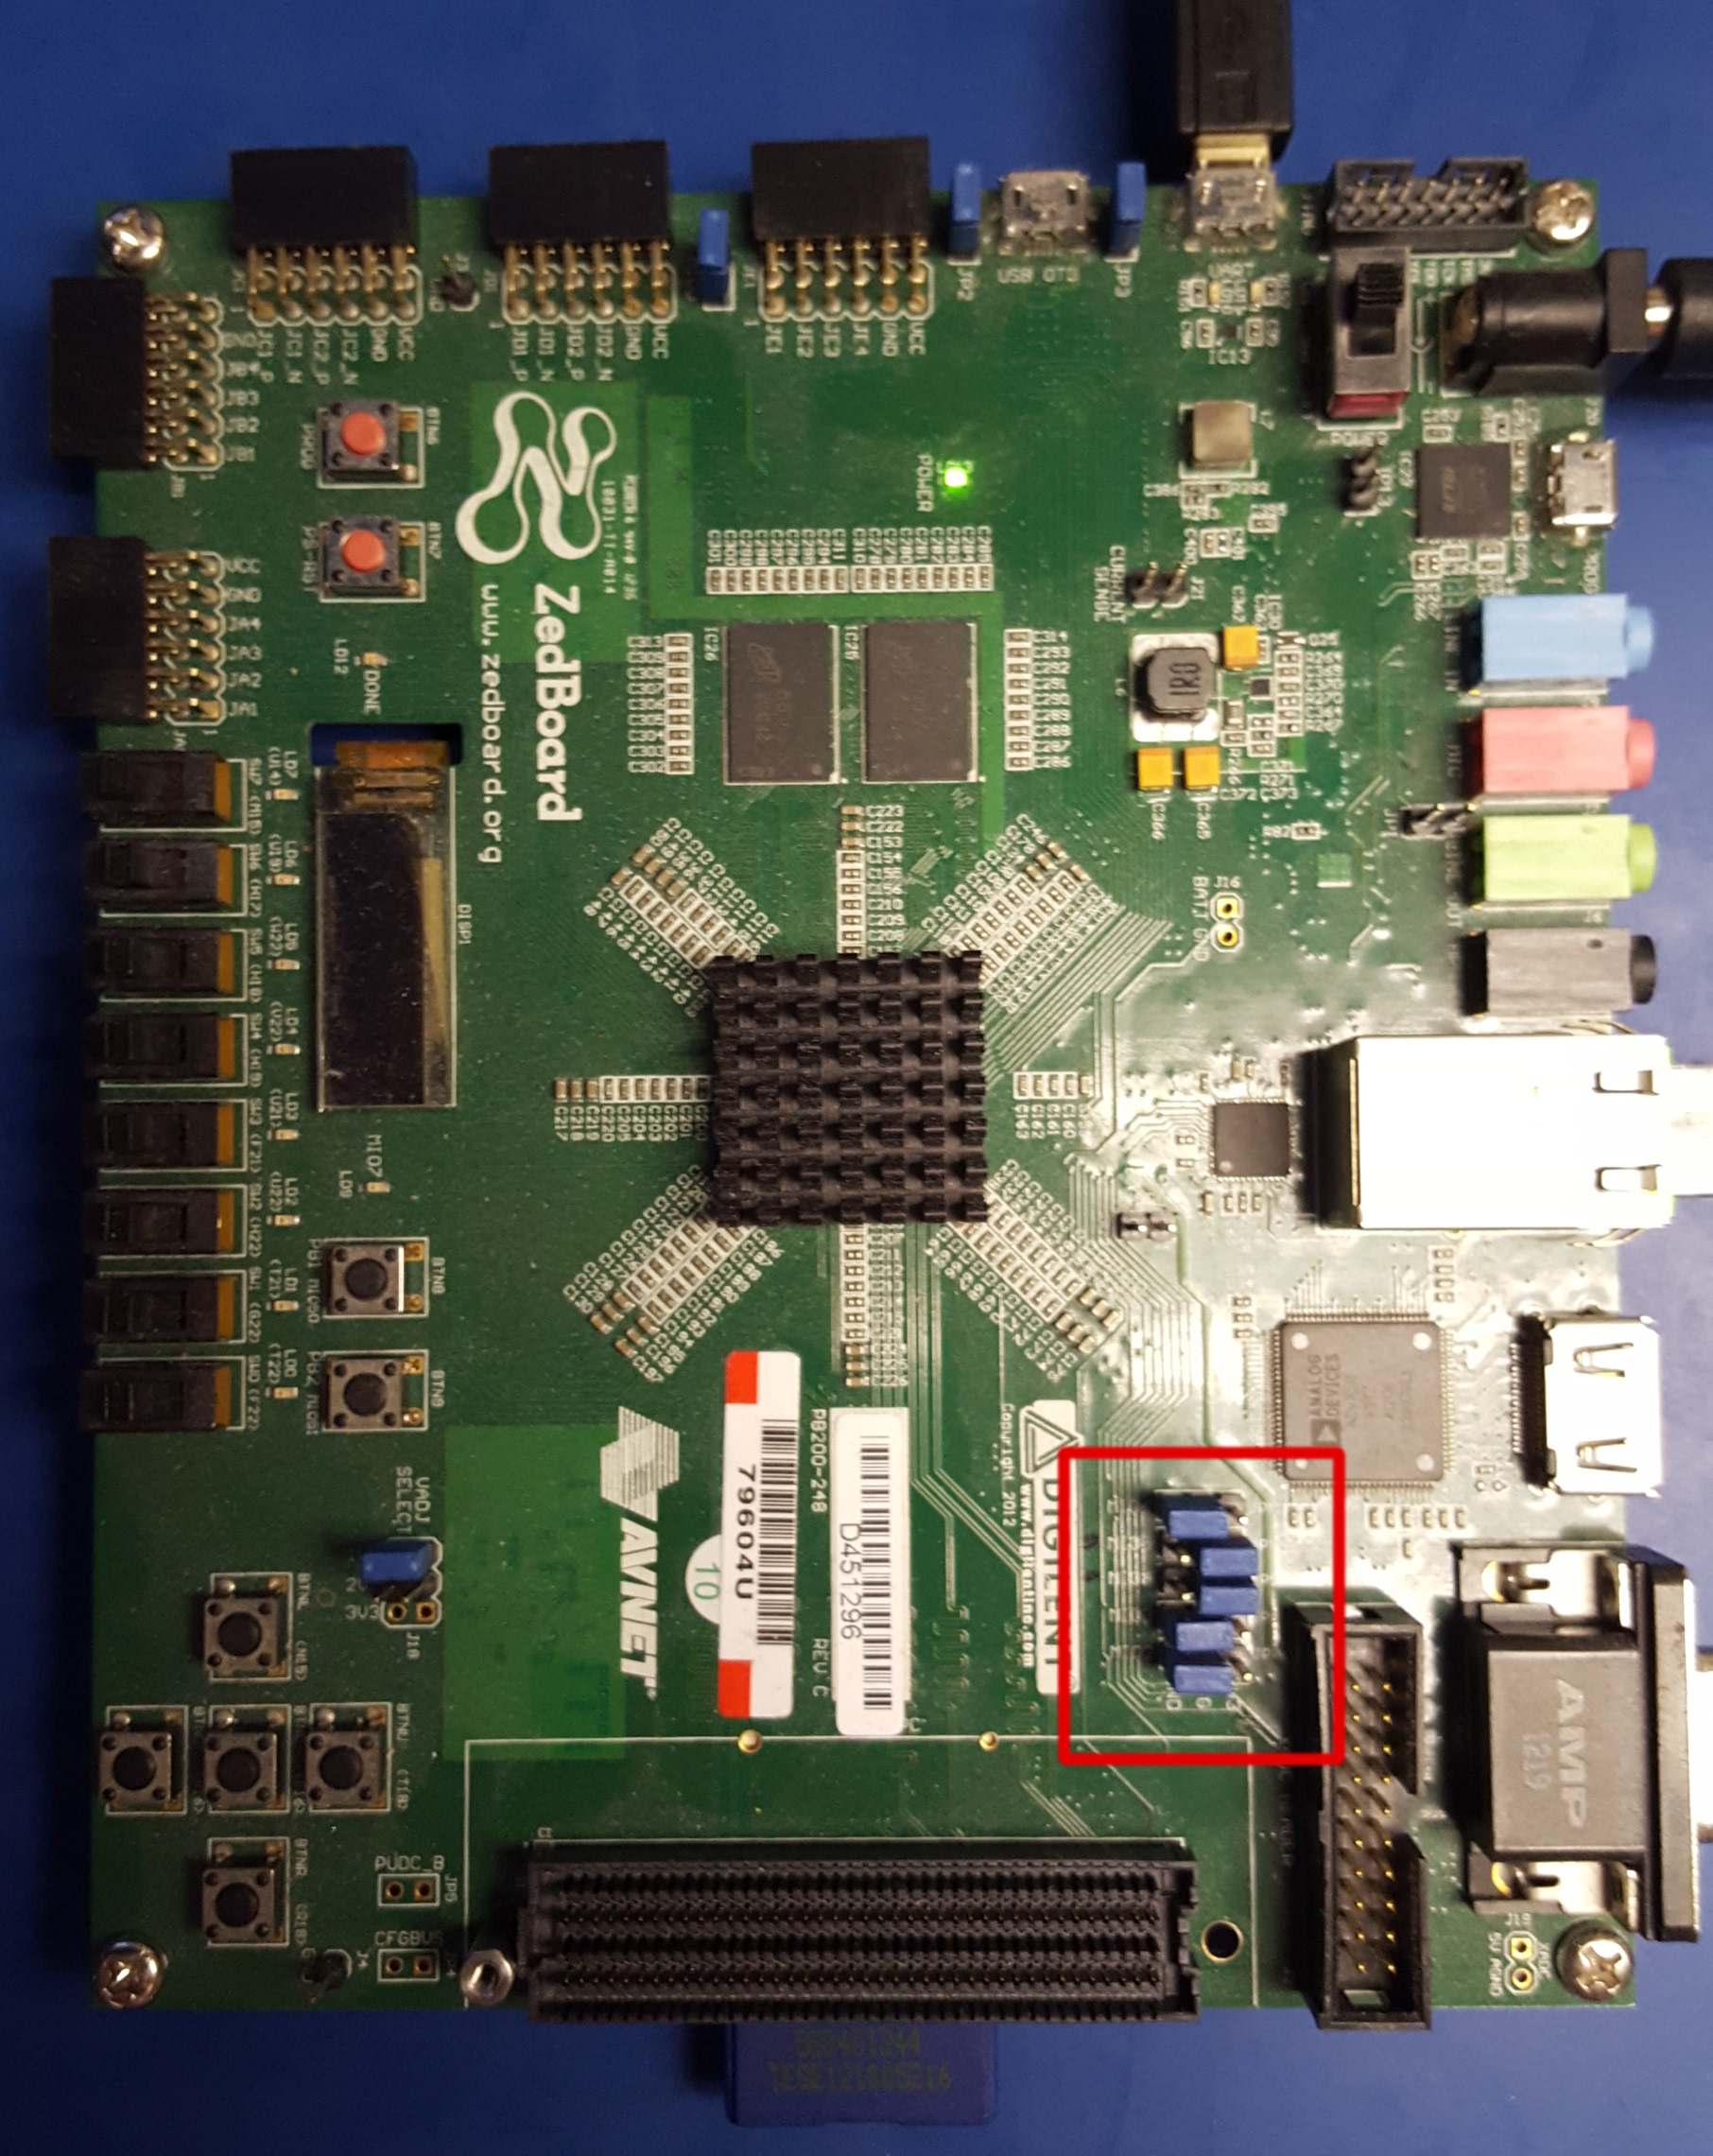
\includegraphics[scale=0.15]{zed_top}}
	\caption{Top View of the ZedBoard with J10, J9, J8 Set}
	\label{fig:zed_top}
\end{figure}
\item The only supported FMC voltage for OpenCPI Zedboard FPGA bitstreams is 2.5 V. To ensure property FMC configuration, the VADJ SELECT (J18) jumper must be set to 2V5.
\end{enumerate}
\item Insert the SD card into the SD card slot.
\item Connect a terminal to the micro-USB connector labelled 'UART' on the ZedBoard. The baud rate should be 115200 baud.
\begin{itemize}
\item per the previous section, ``\texttt{screen /dev/zed0 115200}'' can be used to connect to the serial port.
\end{itemize}
\item Apply power to the ZedBoard with the terminal still connected.
\end{enumerate}

\pagebreak
\section{Development Host Setup - Network Mode ONLY}
% Bring in NFS setup snippet (has subsections)
\input{../../../../../../doc/av/tex/snippets/NFS_Setup_Snippet.tex}
%

\pagebreak
\section{Configuring the run-time environment on the platform}

\subsection{Network Mode}
\begin{enumerate}
\item Ensure the Ethernet cable is plugged in and connected to a network configured for DHCP.
\item Ensure a micro-USB to USB cable is connected between the Zed's serial port and development host.
\item Apply power to the Zedboard
\item Use a serial terminal application to establish a serial connection, for example:

\begin{verbatim}
$ screen /dev/zed0 115200
\end{verbatim}

\item Typically, upon the initial power-on of the platform, the boot sequence will stop at the uboot configuration prompt. When this occurs, simply enter \textit{boot} to allow the boot sequence to continue:
\begin{verbatim}
$ zynq-uboot> boot
\end{verbatim} \medskip

\item After a successful boot to PetaLinux, login to the system, using  ``\textbf{root}`` for user name and password.

\begin{figure}[H]
	\centerline{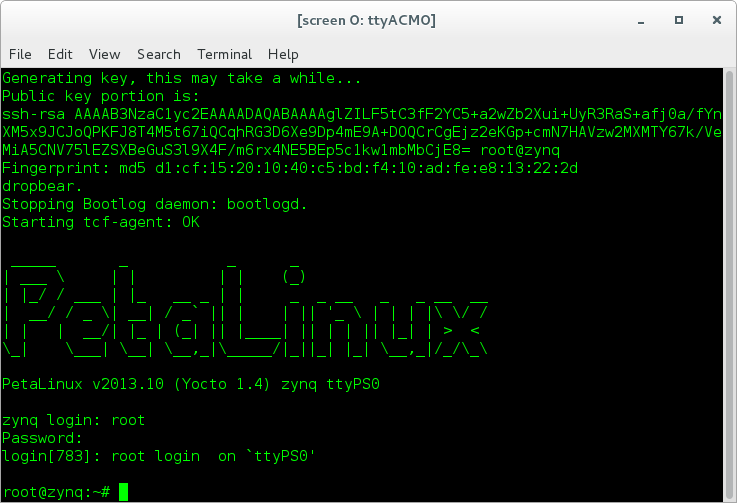
\includegraphics[scale=0.5]{zed_boot}}
	\caption{Successful Boot to PetaLinux}
	\label{fig:boot1}
\end{figure}

\item
\begin{enumerate}
	\item When a \textbf{single} Zedboard is on the network, execute the following command to enable its Ethernet interface:
\begin{verbatim}
$ ifconfig eth0 up
\end{verbatim} \medskip
	\item When \textbf{multiple} Zedboards are on the network, the mynsetsetup.sh script \textbf{MUST} be modified according to \ref{sec:Multiple ZedBoards on the same network} prior to proceeding to the next step, in order to prevent network collisions due to multiple Zedboards having the same MAC address.
\end{enumerate}

\item Setup the OpenCPI environment on remote system

\begin{flushleft}
Each time the SDR is booted, the OpenCPI environment must be setup. By sourcing the \texttt{mynetsetup.sh} script, the remote system's environment is configured for OpenCPI and NFS directories are mounted for Network mode.\footnote{This script calls the \texttt{zynq\_net\_setup.sh} script, which should not be modifiable by the user.}. The user must provide the network address of the development system to the script as its only argument:
\begin{verbatim}
$ source /mnt/card/opencpi/mynetsetup.sh XX.XX.XX.XX
\end{verbatim} \medskip

where XX.XX.XX.XX is the IP address of the NFS host (i.e. that development host, \textit{e.g.} 192.168.1.10). A successful run is shown in Figure~\ref{fig:netsetup}. \medskip

\end{flushleft}

\begin{figure}[H]
	\centerline{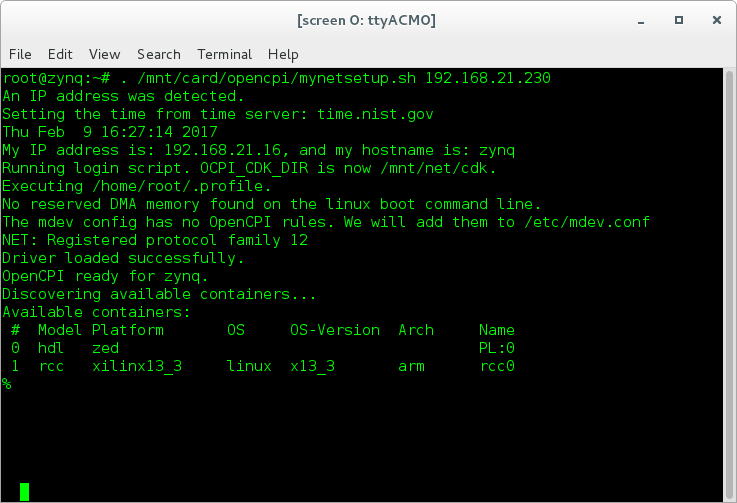
\includegraphics[scale=0.5]{zed_net_setup}}
	\caption{Successful Network Mode Setup}
	\label{fig:netsetup}
\end{figure} \medskip

\input{../../../../../../doc/av/tex/snippets/Ntp_Alarm_Clock.tex}

\end{enumerate}

\pagebreak
\subsection{Standalone Mode}
All artifacts (.so, .bit.gz) for any applications or tests that need to be located on the SD card must be in the \texttt{opencpi/xilinx13\_3/artifacts} folder.  All of the helper utilities such as \texttt{ocpirun} and \texttt{ocpihdl} are already located on the SD card and do not need to be copied over to the ZedBoard platform.

\begin{enumerate}
\item (Not required for OpenCPI in this mode) Plug in an Ethernet cable to a network configured for DHCP.
\item Ensure a micro-USB to USB cable is connected between the Zedboard's serial port and development host.
\item Apply power to the Zedboard
\item Use a serial terminal application to establish a serial connection, for example:

\begin{verbatim}
$ screen /dev/zed0 115200
\end{verbatim} \medskip

\item After a successful boot to PetaLinux, login to the system, using  ``\textbf{root}`` for user name and password.

\begin{figure}[H]
	\centerline{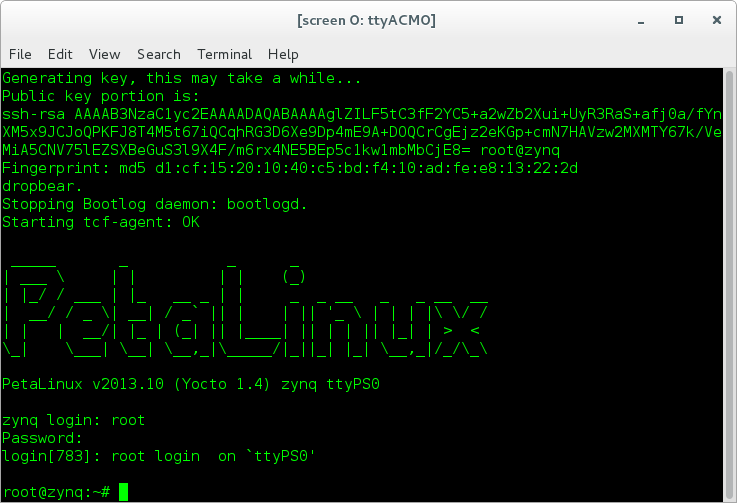
\includegraphics[scale=0.5]{zed_boot}}
	\caption{Successful Boot}
	\label{fig:boot2}
\end{figure}

\item \textcolor{red}{WARNING:}
Applications (including XML-only ones) fail if there is not an IP address assigned to the platform, even when in ``standalone mode.'' When the Ethernet port is not connected to a network configured with DHCP, a temporary IP address must be set:
\begin{verbatim}
$ ifconfig eth0 192.168.244.244
\end{verbatim} \medskip

\item Setup the OpenCPI environment on remote system

Each time the SDR is booted, the OpenCPI environment must be setup. By sourcing the \texttt{mysetup.sh} script, the remote system's environment is configured for OpenCPI.\footnote{This script calls the \texttt{zynq\_setup.sh} script, which should not be modifiable by the user.}. There are no arguments required for this script.
\begin{verbatim}
$ source /mnt/card/opencpi/mysetup.sh
\end{verbatim} \medskip

\noindent A successful setup of the platform will look as follows:
\begin{figure}[H]
	\centerline{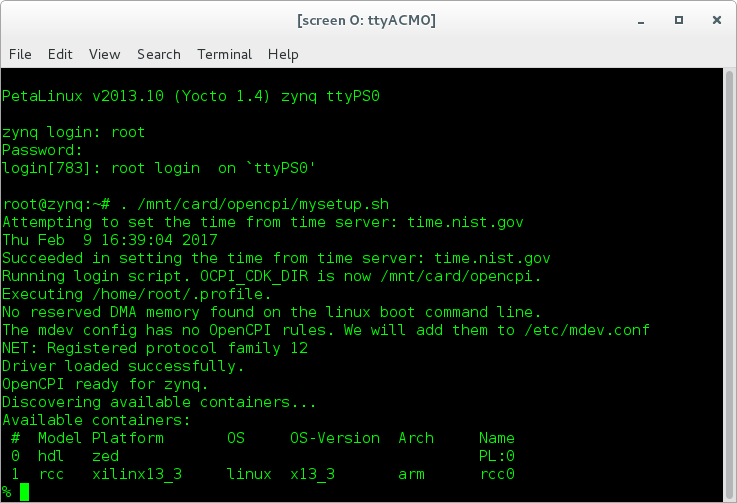
\includegraphics[scale=0.5]{zed_setup}}
	\caption{Successful Standalone Mode Setup}
	\label{fig:standalonesetup}
\end{figure} \medskip

\input{../../../../../../doc/av/tex/snippets/Ntp_Alarm_Clock.tex}

\end{enumerate}

\pagebreak
\section{Build an Application}
\begin{flushleft}
The setup of the platform can be verified by running an application that uses both RCC and HDL workers. A simple application that requires two RCC and one HDL worker is located in \texttt{assets/applications/bias.xml}, but only the RCC artifacts are provided with the installation of RPMs, and are availble on the SD card (Standard Mode) or mounted CDK directory (Network Mode). The remaining task is to build an assembly, or bitstream for loading the FPGA, which contains the HDL worker.
\end{flushleft}

\section{Run an Application}
\subsection{Network Mode}
The default setup script sets the \texttt{OCPI\_LIBRARY\_PATH} variable to include the RCC workers that are required to execute the application, but it must be updated to include to the assembly bitstream that was built.  After running the \texttt{mynetsetup.sh} script, navigate to  \texttt{/mnt/ocpi\_assets/applications}, then update the \texttt{OCPI\_LIBRARY\_PATH} variable:
\begin{verbatim}
$ cd /mnt/card/opencpi/applications
$ export OCPI_LIBRARY_PATH=$OCPI_LIBRARY_PATH:/mnt/ocpi_assets/artifacts
\end{verbatim}
Run the application using the following command:
\begin{verbatim}
$ ocpirun -v -t 1 -d -m bias=hdl bias.xml
\end{verbatim}
The output should be similar to Figure~\ref{fig:netBias}:
\begin{figure}[H]
	\centerline{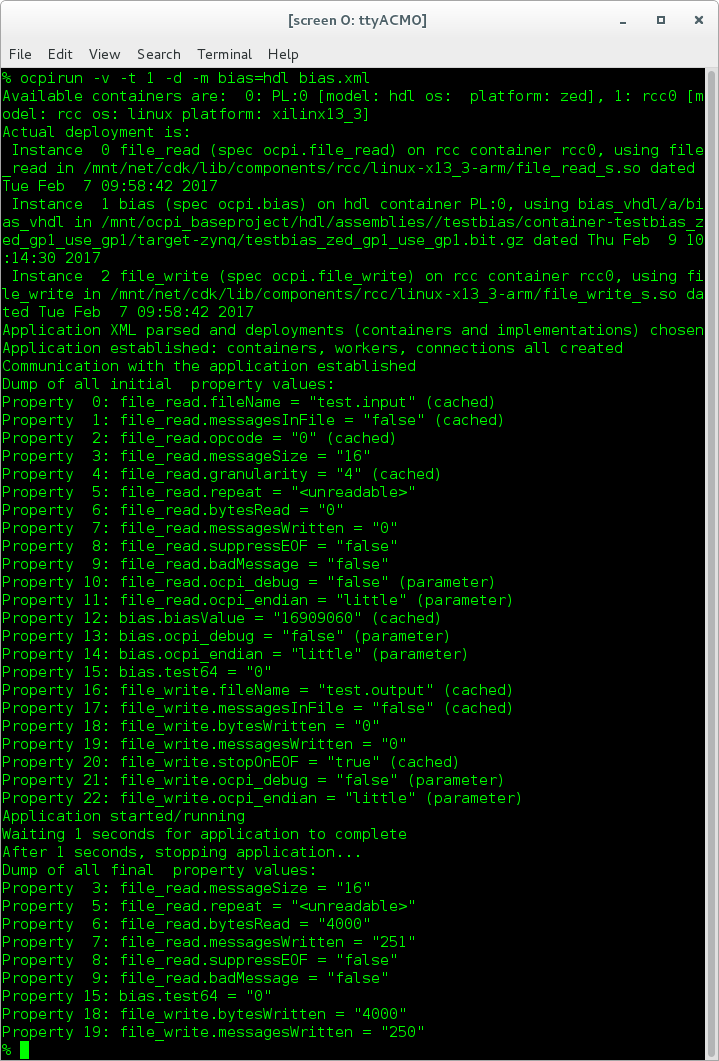
\includegraphics[scale=0.45]{zed_net_bias}}
	\caption{Successful Network Mode Execution}
	\label{fig:netBias}
\end{figure}

\pagebreak
Run the following command to view the input. It should look like Figure~\ref{fig:inBias1}: \\
\begin{verbatim}
$ hexdump test.input | less
\end{verbatim}
\begin{figure}[H]
	\centerline{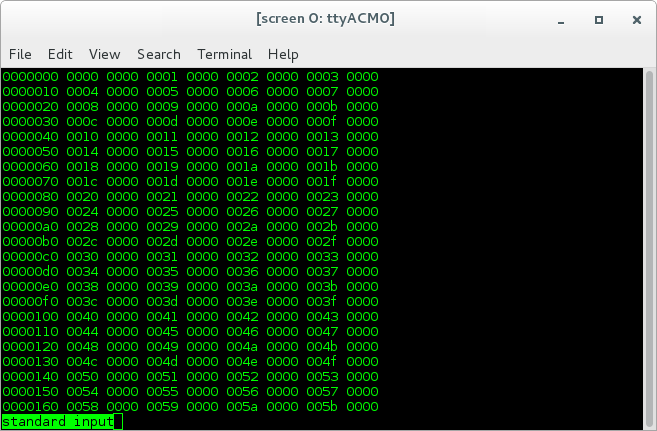
\includegraphics[scale=0.5]{zed_bias_input}}
	\caption{Expected Input}
	\label{fig:inBias1}
\end{figure}

Run the following command to view the output. It should look like Figure~\ref{fig:outBias1}: \\
\begin{verbatim}
$ hexdump test.output | less
\end{verbatim}
\begin{figure}[H]
	\centerline{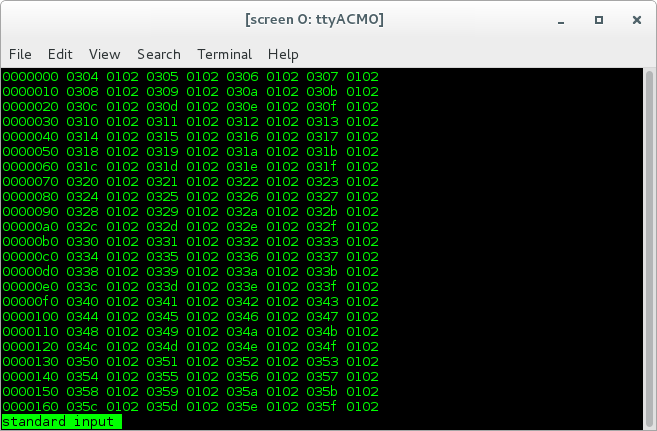
\includegraphics[scale=0.5]{zed_bias_output}}
	\caption{Expected Output}
	\label{fig:outBias1}
\end{figure}

\newpage
\subsection{Standalone Mode}
\begin{flushleft}
The default setup script sets the \texttt{OCPI\_LIBRARY\_PATH} variable to include the all of the artifacts that are required to execute the application. Specifically, all three of the artifacts that are located on the SD card are mounted at \texttt{/mnt/card/opencpi/xilinx13\_3/artifacts}.  After running \texttt{mysetup.sh}, navigate to \texttt{/mnt/card/opencpi/applications} and ensure the \texttt{OCPI\_LIBRARY\_PATH} variable is configure as shown below:
\begin{verbatim}
$ cd /mnt/card/opencpi/applications
$ export OCPI_LIBRARY_PATH=$OCPI_LIBRARY_PATH:/mnt/card/opencpi/xilinx13_3/artifacts
\end{verbatim}

Run the application using the following command:
\begin{verbatim}
$ ocpirun -v -t 1 -d -m bias=hdl bias.xml
\end{verbatim}
The output should be similar to Figure~\ref{fig:standBias}:
\end{flushleft}
\begin{figure}[H]
	\centerline{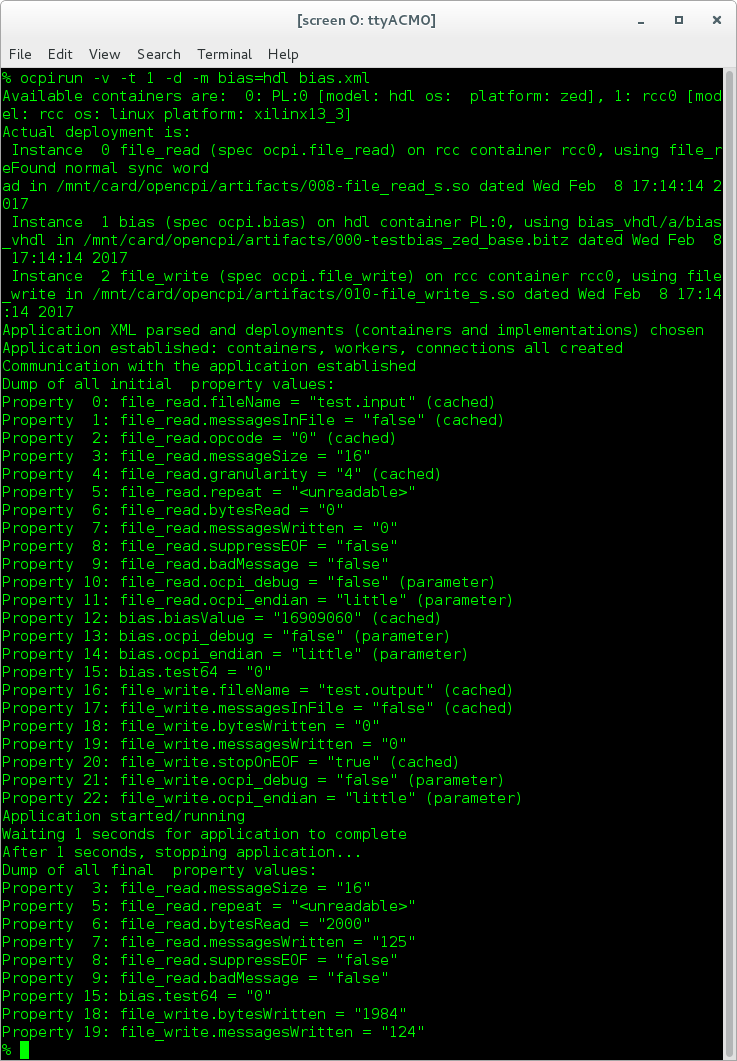
\includegraphics[scale=0.5]{zed_bias}}
	\caption{Successful Standalone Mode Execution}
 \label{fig:standBias}
\end{figure}

\pagebreak
Run the following command to view the input. It should look like Figure~\ref{fig:inBias2}: \\
\begin{verbatim}
$ hexdump test.input | less
\end{verbatim}
\begin{figure}[H]
	\centerline{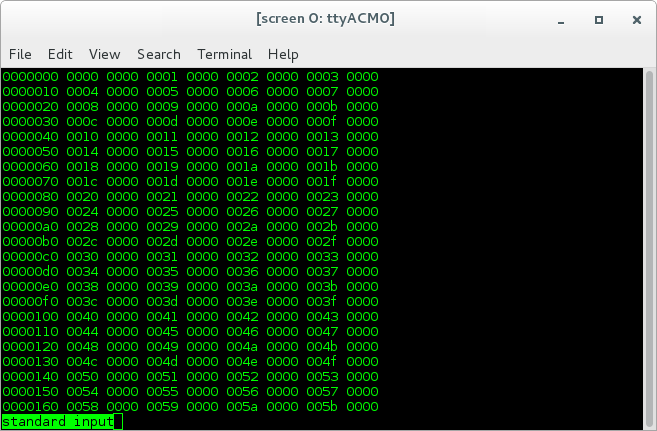
\includegraphics[scale=0.5]{zed_bias_input}}
	\caption{Expected Input}
	\label{fig:inBias2}
\end{figure}

Run the following command to view the output. It should look like Figure~\ref{fig:outBias2}: \\
\begin{verbatim}
$ hexdump test.output | less
\end{verbatim}
\begin{figure}[H]
	\centerline{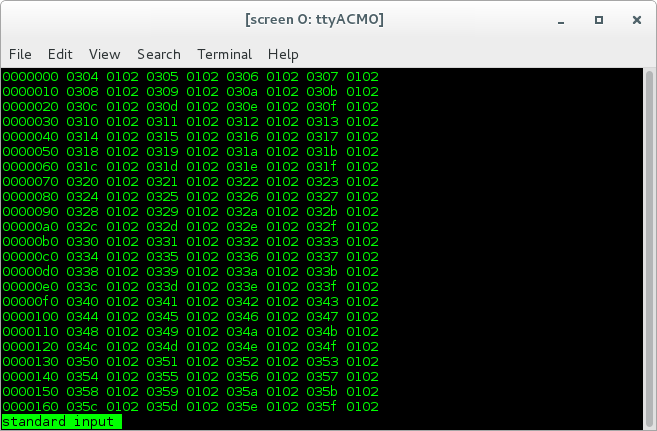
\includegraphics[scale=0.5]{zed_bias_output}}
	\caption{Expected Output}
	\label{fig:outBias2}
\end{figure}

\pagebreak
\begin{appendices}

\section{Using ISE instead of Vivado with the ZedBoard}
\begin{flushleft}
If the user requires the use of the Xilinx ISE tools, rather than the Vivado (recommended), a different OpenCPI platform must be targeted for building bitstreams for the Zedboard. Specifically, the \textit{zed\_ise} (\textit{zynq\_ise} is the target) OpenCPI platform is built using ISE tools, where as the \textit{zed} (\textit{zynq} is the target) OpenCPI platform  is built using Vivado tools.\medskip

Its critical to note that the entire \textit{core} and \textit{assets} projects must be built using ISE tools and that the \textit{zed\_ise} platform is located in the \textit{assets} project.\medskip

After ensuring the proper environment variables are set in support of the ISE tools, use the following command to build from the top-level of a project:

\begin{verbatim}
$ ocpidev build --hdl-platform zed_ise
\end{verbatim}
\end{flushleft}
% Bring in kernel message snippet
\section{Driver Notes}
\input{../../../../../../doc/av/tex/snippets/Driver_Snippet.tex}
%
\end{appendices}
\end{document}
